% Casestudy Eindexamen Oefenen. Bouwen: lualatex casestudy.tex (twee keer).
\documentclass[10.5pt,a4paper]{article}
\usepackage{fontspec}
\usepackage[dutch]{babel}
\usepackage[a4paper,top=24mm,bottom=26mm,inner=25mm,outer=25mm,headsep=8mm,footskip=12mm]{geometry}
\usepackage{xcolor,graphicx,tikz,booktabs,tabularx,enumitem,microtype,fancyhdr,titlesec,xurl,array}
\usepackage[skins]{tcolorbox}
\usepackage{caption,subcaption}
\usetikzlibrary{arrows.meta,positioning,calc}
\usepackage[section]{placeins}
\usepackage{needspace}
\usepackage{float}
\usepackage[hidelinks]{hyperref}

\setmainfont{SourceSerif4}[Extension=.otf,UprightFont=*-Regular,BoldFont=*-Semibold,
  ItalicFont=*-RegularIt,BoldItalicFont=*-SemiboldIt,Numbers=Lining]
\setsansfont{SourceSans3}[Extension=.otf,UprightFont=*-Regular,BoldFont=*-Bold,ItalicFont=*-RegularIt,
  BoldItalicFont=*-BoldIt,FontFace={sb}{n}{*-Semibold},FontFace={k}{n}{*-Black},FontFace={l}{n}{*-Light}]
\newcommand\zwart{\fontseries{k}\selectfont}

\definecolor{petrol}{HTML}{0E6377}
\definecolor{oker}{HTML}{B5651D}
\definecolor{pruim}{HTML}{7A3B69}
\definecolor{groen}{HTML}{3E7B4F}
\definecolor{donker}{HTML}{12313B}
\definecolor{grijs}{HTML}{6B7178}
\definecolor{papier}{HTML}{F4F6F7}
\definecolor{rood}{HTML}{B33A3A}

\linespread{1.12}
\setlength\parindent{0pt}
\setlength\parskip{5pt plus 1pt}
\titleformat{\section}{\needspace{9\baselineskip}\sffamily\zwart\Large\color{donker}}{\color{oker}\thesection}{10pt}{}
\titleformat{\subsection}{\needspace{6\baselineskip}\sffamily\bfseries\large\color{donker}}{\color{oker}\thesubsection}{8pt}{}
\titlespacing*{\section}{0pt}{18pt}{6pt}
\titlespacing*{\subsection}{0pt}{11pt}{4pt}
\captionsetup{font={small,sf},labelfont={bf,color=petrol},labelsep=period,justification=raggedright,singlelinecheck=false}
\captionsetup[sub]{font={footnotesize,sf}}
\setlist{itemsep=2pt,topsep=3pt}

\pagestyle{fancy}\fancyhf{}
\renewcommand\headrulewidth{0pt}
\fancyhead[L]{\sffamily\footnotesize\color{grijs}Promptgestuurde ontwikkeling van een open oefenplatform}
\fancyhead[R]{\sffamily\footnotesize\color{grijs}Jagers \textbullet\ 2026}
\fancyfoot[C]{\sffamily\footnotesize\color{grijs}\thepage}

\tikzset{pijl/.style={-{Stealth[length=2.4mm]},line width=1pt,color=grijs}}
\newcommand\cijfer[3]{%
  \begin{tikzpicture}\node[align=center,font=\sffamily] {{\zwart\fontsize{20}{22}\selectfont\color{#1}#2}\\[1pt]{\scriptsize\color{grijs}#3}};\end{tikzpicture}}

\begin{document}

% =================== titel ===================
\thispagestyle{empty}
\begin{tikzpicture}[remember picture,overlay]
  \fill[donker] (current page.north west) rectangle ($(current page.north east)+(0,-96mm)$);
  \begin{scope}[shift={($(current page.north west)+(0,-96mm)$)}]
    \begin{scope}[white,opacity=.07,line width=.4pt]
      \foreach \i in {0,...,19} {\draw (0,\i*5mm) -- (210mm,\i*5mm);}
      \foreach \i in {0,...,42} {\draw (\i*5mm,0) -- (\i*5mm,96mm);}
    \end{scope}
  \end{scope}
  \foreach \c/\x in {petrol/0,oker/1,pruim/2,groen/3} {\fill[\c] ($(current page.north west)+(25mm+\x*7mm,-20mm)$) rectangle ++(5mm,-5mm);}
  \node[anchor=north west,text=white,align=left,text width=160mm] at ($(current page.north west)+(25mm,-30mm)$)
    {{\sffamily\footnotesize\addfontfeature{LetterSpace=10}CASESTUDY \textbullet\ MENS--AI-SAMENWERKING \textbullet\ CONCEPT, NOVEMBER 2026}\\[4mm]
     {\sffamily\zwart\fontsize{25}{29}\selectfont Promptgestuurde ontwikkeling\\van een open oefenplatform\\voor centrale examens}\\[4mm]
     {\sffamily\fontsize{12.5}{16}\selectfont\hyphenpenalty=10000\color{white!80!petrol} Een casestudy naar iteratieve samenwerking tussen een domeinexpert en een AI-agent}};
  \node[anchor=south west,text=white,align=left] at ($(current page.north west)+(25mm,-89mm)$)
    {\sffamily\small\bfseries Jesse Jagers \quad{\mdseries\color{white!75!petrol} ontwikkeld met Claude Code (Anthropic)}};
\end{tikzpicture}
\vspace*{82mm}

\begin{tcolorbox}[enhanced,colback=white,colframe=petrol!30,boxrule=.5pt,arc=0pt,left=12pt,right=12pt,top=8pt,bottom=8pt,fontupper=\small]
{\sffamily\bfseries\color{petrol}Abstract.}\enspace
Dutch national examination papers are public, yet topic-based practice material is predominantly commercial. This case study
examines whether a complete, free practice platform can be realised by a single domain expert who instructs an AI agent
exclusively in natural language. Over six days, the collaboration produced a web platform with 4{,}748 official examination
items for mathematics and the natural sciences, classified by syllabus subdomain and linked to the official marking scheme,
together with eleven print-ready examination books (2{,}916 pages). We describe the division of roles, the iteration cycle,
the system architecture and the quality-assurance mechanisms. The results indicate that natural-language instruction suffices
for implementation, provided that requirements are measurable, defects are remedied at the level of the system rather than
the instance, and every observed defect is converted into an automated check.

\medskip
{\sffamily\bfseries\color{petrol}Samenvatting.}\enspace
Deze casestudy onderzoekt of één domeinexpert, uitsluitend via instructies in natuurlijke taal aan een AI-agent, een volledig
gratis oefenplatform voor de centrale examens kan realiseren. Binnen zes dagen ontstonden een website met 4.748 officiële
examenvragen, ingedeeld naar syllabus en gekoppeld aan het correctievoorschrift, en elf drukklare examenbundels. De
bevindingen wijzen op vier randvoorwaarden: meetbare eisen, herstel op systeemniveau, automatische verificatie en
menselijke beoordeling van het eindresultaat.
\end{tcolorbox}

\begin{center}
\cijfer{petrol}{4.748}{examenvragen}\hspace{5mm}\cijfer{oker}{11}{vakken havo/vwo}\hspace{5mm}\cijfer{pruim}{2.916}{pagina's in bundels}\hspace{5mm}\cijfer{groen}{0}{regels code door de mens}\hspace{5mm}\cijfer{donker}{6}{dagen}
\end{center}

% =================== 1 ===================
\section{Inleiding}

De opgaven en correctievoorschriften van de centrale examens worden jaarlijks door het College voor Toetsen en Examens
(CvTE) openbaar gemaakt en mogen met bronvermelding worden hergebruikt \cite{copyright}. De meerwaarde van commercieel
oefenmateriaal ligt daarom niet in de opgaven zelf, maar in de ordening ervan: het groeperen van vragen per onderwerp, het
koppelen aan antwoordmodellen en het drukklaar opmaken. Die ordening is arbeidsintensief, wat verklaart waarom
examenbundels en examentrainingen doorgaans betaald zijn; trainingen kosten circa \texteuro\,375--390 per vak \cite{markt}.

Recente AI-agents kunnen niet alleen tekst genereren, maar ook bestanden lezen en schrijven, programma's uitvoeren en
resultaten visueel inspecteren \cite{claude}. Dat roept de vraag op of het ordeningswerk volledig kan worden gedelegeerd,
terwijl de mens de rol van opdrachtgever en eindredacteur behoudt. Deze studie behandelt twee onderzoeksvragen:

\begin{enumerate}[label=\textbf{OV\arabic*},leftmargin=3em]
  \item In hoeverre kan een functioneel oefenplatform met drukklare examenbundels worden gerealiseerd uitsluitend door
        instructies in natuurlijke taal?
  \item Welke randvoorwaarden bepalen de kwaliteit van het resultaat?
\end{enumerate}

% =================== 2 ===================
\section{Methode}

\subsection{Onderzoeksopzet}
De studie is opgezet als een enkelvoudige, ontwerpgerichte casestudy. De ontwikkeling vond plaats van 4 tot en met
9 november 2026. Als gegevensbronnen dienen de versiegeschiedenis van de broncode, de gevoerde instructies, de automatisch
gegenereerde controleverslagen en de tussentijdse producten (pdf's en schermafbeeldingen). De auteur, bijlesdocent en
vertrouwd met de examens, trad op als opdrachtgever; de AI-agent \emph{Claude Code} voerde alle implementatie uit. De
auteur schreef zelf geen programmacode.

\subsection{Rolverdeling}
Figuur~\ref{fig:rollen} vat de rolverdeling samen. De mens bepaalt \emph{wat} er moet ontstaan en \emph{of} het goed is;
de agent bepaalt \emph{hoe} het ontstaat en toont aan \emph{dat} het voldoet aan de gestelde eisen.

\begin{figure}[!htb]
\centering
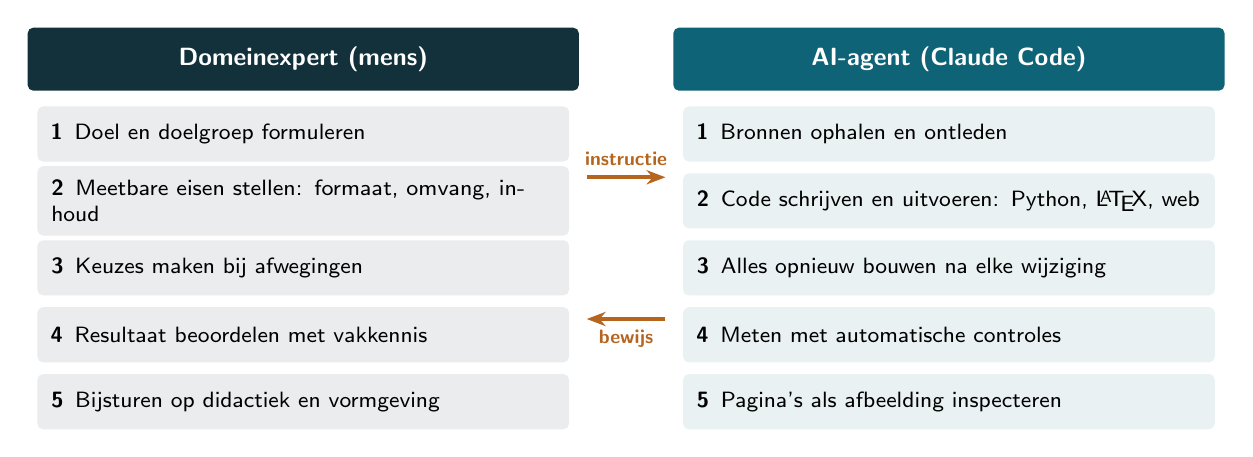
\begin{tikzpicture}[
  kop/.style={font=\sffamily\bfseries\small,text=white,fill=#1,minimum width=70mm,minimum height=8mm,rounded corners=2pt},
  taak/.style={font=\sffamily\footnotesize,fill=#1!9,text width=64mm,inner sep=5pt,rounded corners=2pt,align=left,minimum height=7mm}]
  \node[kop=donker] at (0,0) {Domeinexpert (mens)};
  \node[kop=petrol] at (82mm,0) {AI-agent (Claude Code)};
  \foreach \t [count=\i] in {Doel en doelgroep formuleren,{Meetbare eisen stellen: formaat, omvang, inhoud},Keuzes maken bij afwegingen,Resultaat beoordelen met vakkennis,Bijsturen op didactiek en vormgeving}
    \node[taak=donker] at (0,-\i*8.5mm-1mm) {\textbf{\i}\enspace\t};
  \foreach \t [count=\i] in {Bronnen ophalen en ontleden,{Code schrijven en uitvoeren: Python, \LaTeX, web},Alles opnieuw bouwen na elke wijziging,Meten met automatische controles,Pagina's als afbeelding inspecteren}
    \node[taak=petrol] at (82mm,-\i*8.5mm-1mm) {\textbf{\i}\enspace\t};
  \draw[pijl,color=oker,line width=1.5pt] (36mm,-15mm) -- node[above,font=\sffamily\scriptsize\bfseries,text=oker]{instructie} (46mm,-15mm);
  \draw[pijl,color=oker,line width=1.5pt] (46mm,-33mm) -- node[below,font=\sffamily\scriptsize\bfseries,text=oker]{bewijs} (36mm,-33mm);
\end{tikzpicture}
\caption{Rolverdeling tussen domeinexpert en AI-agent. De mens levert eisen en oordelen; de agent levert implementatie en
het bewijs dat aan de eisen is voldaan.}
\label{fig:rollen}
\end{figure}

\subsection{Iteratiecyclus}
Het werk verliep in korte iteraties volgens een vaste cyclus (figuur~\ref{fig:cyclus}). Kenmerkend is de terugkoppeling:
een waargenomen defect wordt niet op één plaats hersteld, maar leidt tot een aanpassing van de regels en tot een nieuwe
automatische controle die voor alle vakken geldt. Na elke iteratie werden alle producten opnieuw gegenereerd.

\begin{figure}[!htb]
\centering
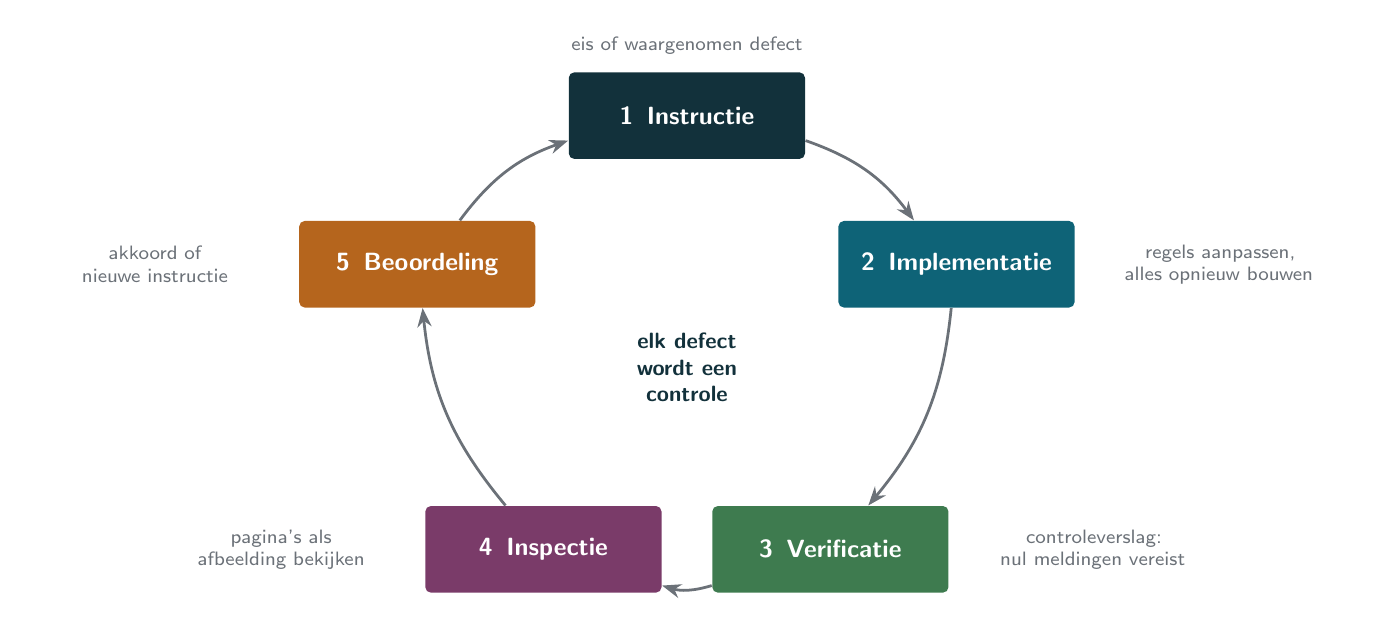
\begin{tikzpicture}[
  stap/.style={draw=none,fill=#1,text=white,font=\sffamily\small\bfseries,minimum width=30mm,minimum height=11mm,align=center,rounded corners=2pt},
  noot/.style={font=\sffamily\scriptsize,text=grijs,align=center,text width=30mm}]
  \node[stap=donker] (v) at (90:30mm) {1\enspace Instructie};
  \node[stap=petrol] (b) at (18:36mm) {2\enspace Implementatie};
  \node[stap=groen] (m) at (-54:31mm) {3\enspace Verificatie};
  \node[stap=pruim] (k) at (-126:31mm) {4\enspace Inspectie};
  \node[stap=oker] (s) at (162:36mm) {5\enspace Beoordeling};
  \foreach \a/\b in {v/b,b/m,m/k,k/s,s/v} \draw[pijl] (\a) to[bend left=17] (\b);
  \node[noot,above=1mm of v] {eis of waargenomen defect};
  \node[noot,right=2mm of b] {regels aanpassen,\\alles opnieuw bouwen};
  \node[noot,right=2mm of m] {controleverslag:\\nul meldingen vereist};
  \node[noot,left=2mm of k] {pagina's als\\afbeelding bekijken};
  \node[noot,left=2mm of s] {akkoord of\\nieuwe instructie};
  \node[font=\sffamily\footnotesize\bfseries,text=donker,align=center] at (0,-2mm) {elk defect\\wordt een\\controle};
\end{tikzpicture}
\caption{De iteratiecyclus. Stap 2 tot en met 4 voert de agent uit; stap 5 blijft een menselijk oordeel.}
\label{fig:cyclus}
\end{figure}

\subsection{Typen instructies}
De instructies worden hier niet letterlijk weergegeven, maar ingedeeld in vijf typen (figuur~\ref{fig:prompts}). Aan het
begin overheerste \emph{specificatie}; naarmate het product rijper werd, verschoof het zwaartepunt naar \emph{correctie},
\emph{verfijning} en \emph{validatie}. Instructies van het type \emph{strategie} kwamen op beslismomenten, zoals de keuze
tussen uitbreiden en toespitsen.

\begin{figure}[!htb]
\centering
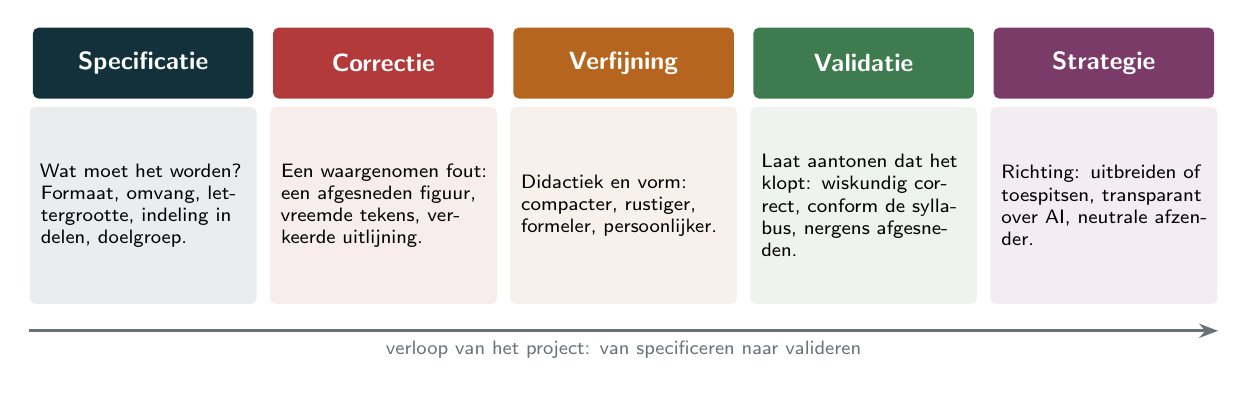
\begin{tikzpicture}[
  type/.style={fill=#1,text=white,font=\sffamily\small\bfseries,minimum width=28mm,minimum height=9mm,rounded corners=2pt},
  vb/.style={fill=#1!9,font=\sffamily\scriptsize,text width=26mm,inner sep=4pt,align=left,rounded corners=2pt,minimum height=25mm}]
  \foreach \k/\t/\v [count=\i] in {
      donker/Specificatie/{Wat moet het worden? Formaat, omvang, lettergrootte, indeling in delen, doelgroep.},
      rood/Correctie/{Een waargenomen fout: een afgesneden figuur, vreemde tekens, verkeerde uitlijning.},
      oker/Verfijning/{Didactiek en vorm: compacter, rustiger, formeler, persoonlijker.},
      groen/Validatie/{Laat aantonen dat het klopt: wiskundig correct, conform de syllabus, nergens afgesneden.},
      pruim/Strategie/{Richting: uitbreiden of toespitsen, transparant over AI, neutrale afzender.}} {
    \node[type=\k] at (\i*30.5mm,0) {\t};
    \node[vb=\k,anchor=north] at (\i*30.5mm,-5.5mm) {\v};
  }
  \draw[pijl] (16mm,-34mm) -- node[below,font=\sffamily\scriptsize,text=grijs]{verloop van het project: van specificeren naar valideren} (167mm,-34mm);
\end{tikzpicture}
\caption{Indeling van de instructies naar type, met kenmerkende voorbeelden (geparafraseerd).}
\label{fig:prompts}
\end{figure}

% =================== 3 ===================
\section{Systeemontwerp}

\subsection{Datapijplijn}
Figuur~\ref{fig:pijplijn} toont de pijplijn van brondocument naar eindproduct, met de omvang per stap. Website en bundels
delen dezelfde ontleding; daardoor werkt elke verbetering in de ontleding door in beide producten.

\begin{figure}[!htb]
\centering
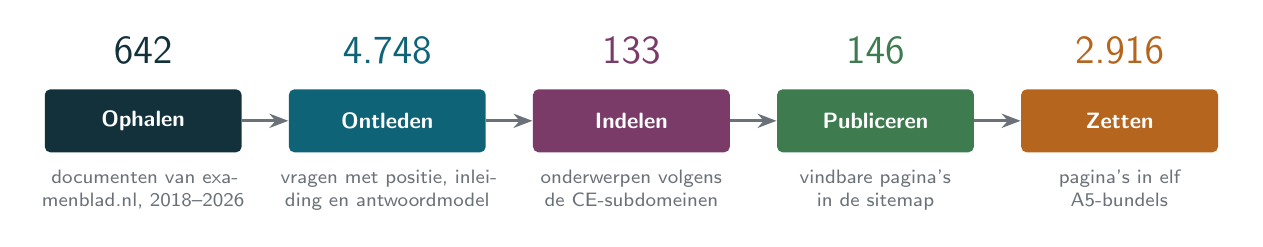
\begin{tikzpicture}[
  stap/.style={fill=#1,text=white,font=\sffamily\footnotesize\bfseries,minimum width=25mm,minimum height=8mm,rounded corners=2pt},
  getal/.style={font=\sffamily\zwart\fontsize{15}{16}\selectfont,text=#1},
  uitleg/.style={font=\sffamily\scriptsize,text=grijs,align=center,text width=27mm}]
  \foreach \k/\t/\g/\u [count=\i] in {
      donker/Ophalen/642/{documenten van examenblad.nl, 2018--2026},
      petrol/Ontleden/4.748/{vragen met positie, inleiding en antwoordmodel},
      pruim/Indelen/133/{onderwerpen volgens de CE-subdomeinen},
      groen/Publiceren/146/{vindbare pagina's in de sitemap},
      oker/Zetten/2.916/{pagina's in elf A5-bundels}} {
    \node[getal=\k] at (\i*31mm,9mm) {\g};
    \node[stap=\k] (s\i) at (\i*31mm,0) {\t};
    \node[uitleg,below=1mm of s\i] {\u};
  }
  \foreach \i/\j in {1/2,2/3,3/4,4/5} \draw[pijl] (s\i) -- (s\j);
\end{tikzpicture}
\caption{De pijplijn met de omvang per stap. Publiceren en zetten gebruiken dezelfde uitsneden: op de website als afbeelding,
in de bundels als vectoruitsnede.}
\label{fig:pijplijn}
\end{figure}

Bij het \emph{ontleden} worden tekstregels met hun positie uit de pdf gelezen. Vragen worden herkend aan het patroon
\emph{punten -- vraagnummer} in de kantlijn, antwoorden aan \emph{vraagnummer -- maximumscore}. Een rasteranalyse van elke
pagina onderscheidt tekst van tekening, zodat een vraag uitsluitend op een witte regel wordt gesneden en nooit door een figuur.

\subsection{Indeling naar syllabus en validatie}
Elke vraag is door de agent afzonderlijk gelezen, met inleiding en antwoordmodel, en toegewezen aan het subdomein waarop
zij het sterkst betrekking heeft; de auteur keek daarbij mee. Na afronding is de indeling op twee niveaus gevalideerd
tegen de officiële examenstof:

\begin{itemize}
  \item \textbf{Structuur.} Voor alle elf vakken is de tabel \emph{Domeinindeling en CE-toekenning} uit de syllabus 2026
        uitgelezen. Bij wiskunde en natuurkunde vielen alle onderwerpen binnen de CE-subdomeinen. Bij scheikunde droegen
        enkele onderwerpen de code van een subdomein dat alleen in het schoolexamen wordt getoetst; bij biologie havo was
        één onderwerp (voortplanting) geheel schoolexamenstof. Deze afwijkingen zijn hersteld (tabel~\ref{tab:validatie}).
  \item \textbf{Vraag.} In een aselecte steekproef van 49 vragen uit zeven vakken stonden 48 vragen bij een passend
        onderwerp; één geval was twijfelachtig.
\end{itemize}

\begin{table}[!htb]
\centering\small
\begin{tabularx}{\linewidth}{@{}l l X@{}}
\toprule
\sffamily\bfseries Vak & \sffamily\bfseries Bevinding & \sffamily\bfseries Maatregel \\
\midrule
Wiskunde (5) & conform & geen \\
Natuurkunde (2) & conform & geen \\
Scheikunde (2) & codes C5, C7, C8 alleen SE & codes vervangen door de sferen uit de syllabus 2026 \\
Biologie havo & \emph{voortplanting} alleen SE & onderwerp opgeheven; 14 vragen heringedeeld naar CE-onderwerpen \\
Biologie vwo & havo-nummering gebruikt & eigen vwo-nummering; eiwitsynthese en voortplanting zijn daar CE \\
\bottomrule
\end{tabularx}
\caption{Validatie van de indeling tegen de CE-toekenning in de syllabi. De inhoudsopgave van een commerciële examenbundel
biologie markeert voortplanting eveneens als schoolexamenstof \cite{bundel}.}
\label{tab:validatie}
\end{table}

\subsection{Kwaliteitscriteria voor een examenbundel}
Een bruikbare examenbundel stelt eisen die verder gaan dan het bijeenbrengen van opgaven. Tabel~\ref{tab:criteria} geeft de
criteria die tijdens het project zijn geëxpliciteerd en de wijze waarop elk criterium technisch is geborgd.

\begin{table}[!htb]
\centering\small
\begin{tabularx}{\linewidth}{@{}>{\sffamily\bfseries}p{29mm} X X@{}}
\toprule
\normalfont\sffamily\bfseries Criterium & \sffamily\bfseries Eis & \sffamily\bfseries Borging \\
\midrule
Getrouwheid & opgaven en antwoorden ongewijzigd & vectoruitsneden uit de originele pdf; niets overgetypt \\
Leesbaarheid & tekst 10--13\,pt & schaal $\approx 0{,}84$ (12 naar 10\,pt); melding onder 90\,\% \\
Omvang & hooguit 280 pagina's A5 & paginabudget; het oudste examen vervalt bij overschrijding \\
Volledigheid & elke vraag en elk antwoord aanwezig & telling: aantal vragen gelijk aan aantal antwoorden \\
Integriteit van figuren & niets afgesneden of gesplitst & meting van inkt buiten de snijlijn; naadloze aansluiting \\
Navigeerbaarheid & per onderwerp, nummering per onderwerp & indeling naar syllabus; verwijzingen naar de uitwerkingen \\
Typografie & uitlijning, afbreking, alle tekens & uitlijning op tekstbegin; Nederlandse afbreekregels; glyphcontrole \\
Herkomst & bron en hergebruik vermeld & colofon en bronvermelding per examen \\
\bottomrule
\end{tabularx}
\caption{Kwaliteitscriteria voor een examenbundel en de technische borging ervan. Een bundel geldt als gereed bij nul
meldingen in het controleverslag, gevolgd door visuele inspectie.}
\label{tab:criteria}
\end{table}

% =================== 4 ===================
\section{Resultaten}

\subsection{Iteraties en foutklassen}
De kwaliteit van de bundels ontstond grotendeels in de iteraties na de eerste versie. Tabel~\ref{tab:iteraties} groepeert de
belangrijkste iteraties naar aanleiding, foutklasse en systeemmaatregel. Elke maatregel werd generiek geformuleerd, zodat
zij voor alle vakken gold, en werd vergezeld van een controle die herhaling signaleert.

\begin{table}[!htb]
\centering\small
\begin{tabularx}{\linewidth}{@{}>{\sffamily\bfseries}p{22mm} X X@{}}
\toprule
\normalfont\sffamily\bfseries Type & \sffamily\bfseries Foutklasse & \sffamily\bfseries Systeemmaatregel \\
\midrule
Correctie & figuren links buiten de snijlijn & snijlijn per blok verbreed tot de figuur volledig is opgenomen (fig.~\ref{fig:snij}) \\
Correctie & figuur naast tekst gesplitst over twee vragen & stukken sluiten naadloos aan, zonder paginabreuk \\
Correctie & exponent gescheiden van formule & grens schuift langs korte tekstfragmenten (fig.~\ref{fig:formule}) \\
Correctie & vreemde tekens in de bronvermelding & aanvullingen uitgesloten; tekens genormaliseerd \\
Correctie & tabelcel gelezen als vraagnummer & vraagnummers moeten oplopen \\
Verfijning & witruimte en nummering & compactere uitwerkingen; nummering per onderwerp \\
Validatie & omslag wiskundig onjuist & tekening herberekend: raak- en snijpunten exact (fig.~\ref{fig:omslag}) \\
Validatie & indeling wijkt af van CE-toekenning & codes en onderwerpen aangepast (tabel~\ref{tab:validatie}) \\
\bottomrule
\end{tabularx}
\caption{Belangrijkste iteraties naar type instructie, foutklasse en generieke maatregel.}
\label{tab:iteraties}
\end{table}

\begin{figure}[!htb]
\centering
\begin{subfigure}[t]{.53\linewidth}\centering
  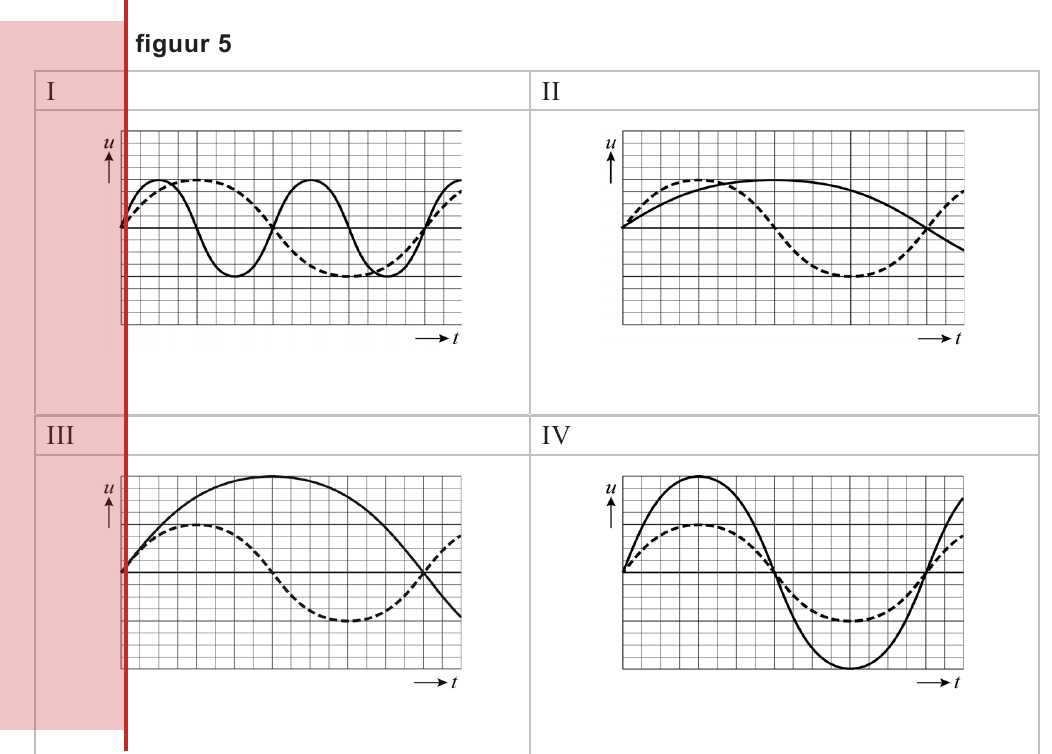
\includegraphics[width=\linewidth]{fig/snij-voor.png}
  \caption{Origineel; alles links van de rode lijn viel buiten de uitsnede.}
\end{subfigure}\hfill
\begin{subfigure}[t]{.43\linewidth}\centering
  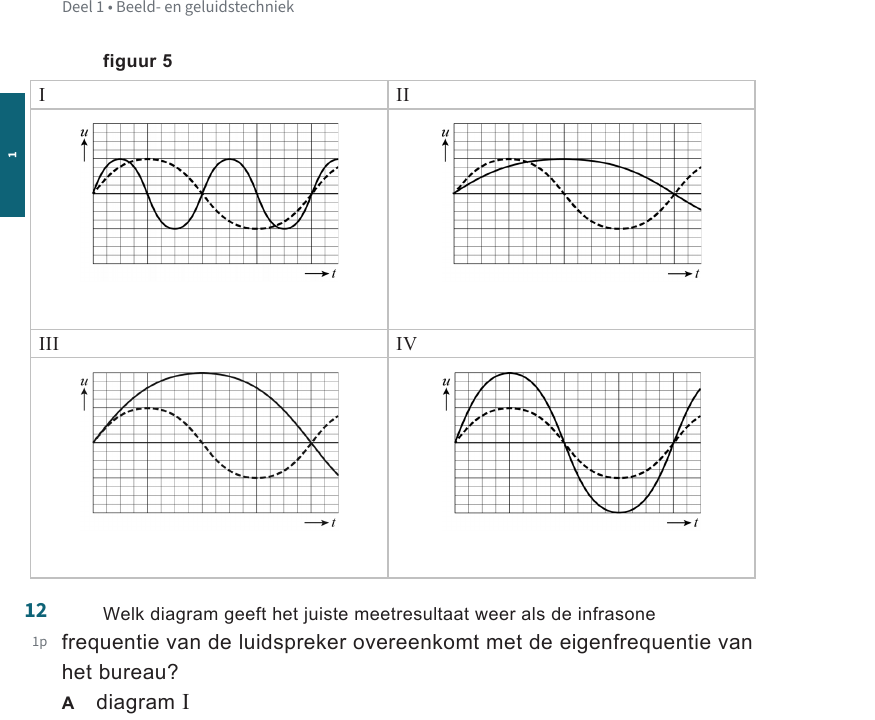
\includegraphics[width=\linewidth]{fig/snij-na.png}
  \caption{In de bundel na de systeemmaatregel.}
\end{subfigure}
\caption{Foutklasse \emph{figuur buiten de snijlijn} (natuurkunde havo 2024-I, figuur 5).}
\label{fig:snij}
\end{figure}

\begin{figure}[!htb]
\centering
\begin{minipage}[b]{.43\linewidth}\centering
  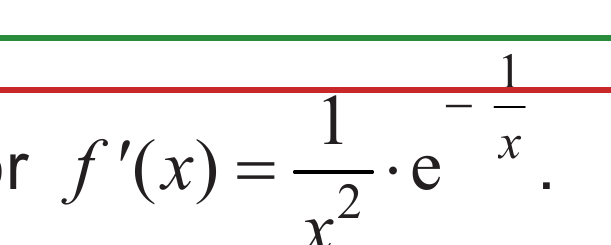
\includegraphics[width=\linewidth]{fig/formule-grens.png}
  \captionof{figure}{Foutklasse \emph{exponent gescheiden}: oude grens (rood) en nieuwe grens (groen) in $e^{-1/x}$.}
  \label{fig:formule}
\end{minipage}\hfill
\begin{minipage}[b]{.53\linewidth}\centering
  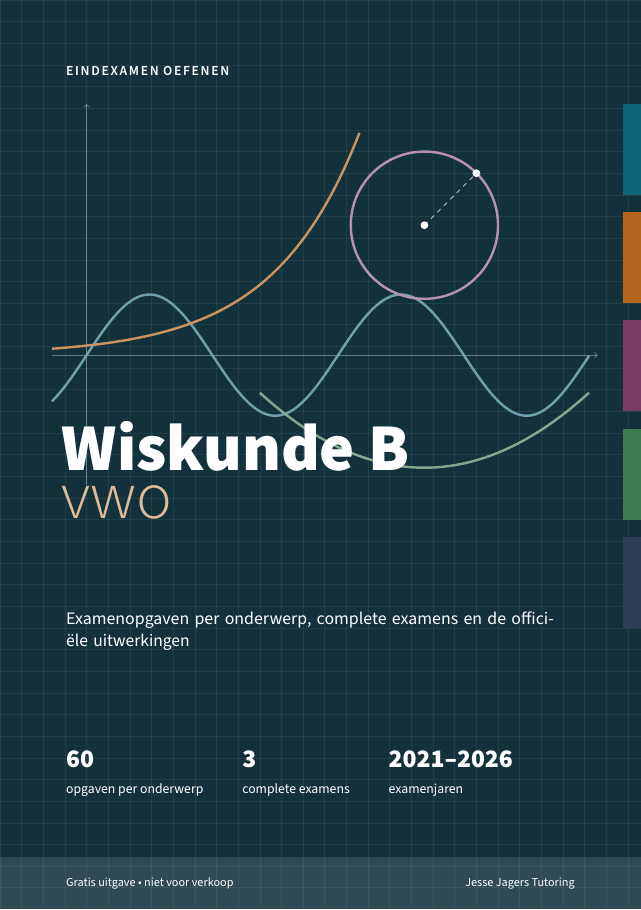
\includegraphics[width=.485\linewidth,trim=0 330 0 0,clip]{fig/omslag-oud.png}\hfill
  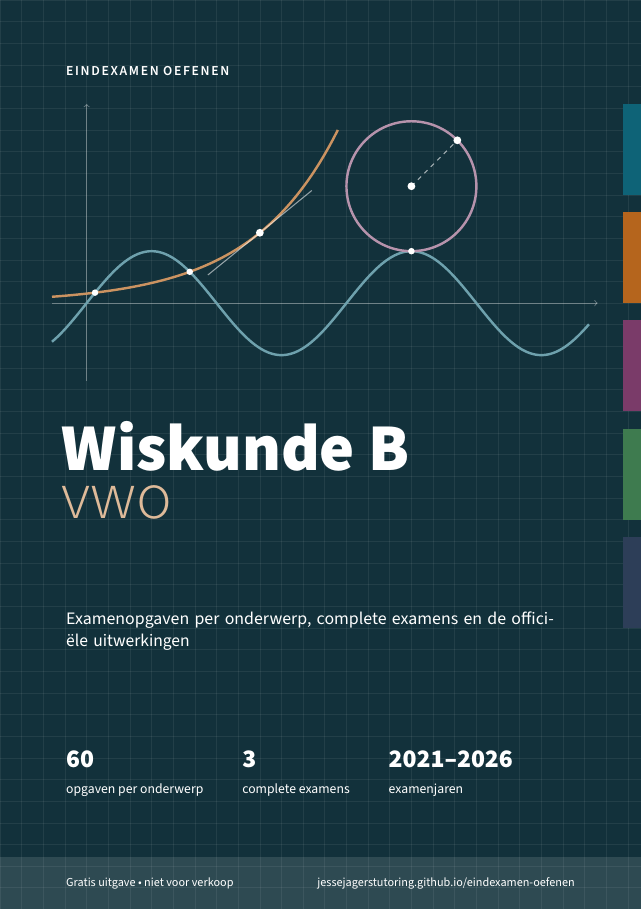
\includegraphics[width=.485\linewidth,trim=0 330 0 0,clip]{fig/omslag-nieuw.png}
  \captionof{figure}{Omslag voor (links) en na validatie (rechts): de cirkel raakt $y=12\sin(6x)$ in de top; de raaklijn aan $y=2{,}2e^{x/20}$ in $x=40$ heeft helling $0{,}8128$.}
  \label{fig:omslag}
\end{minipage}
\end{figure}

\subsection{Kwantitatieve uitkomsten}

\begin{table}[!htb]
\centering\small
\begin{tabular}{@{}lr@{}}
\toprule
Examenvragen, ingedeeld en gekoppeld aan het correctievoorschrift & 4.748 \\
Vakken (havo en vwo) / examens per vak & 11 / 16 \\
Examenbundels / totaal aantal pagina's & 11 / 2.916 \\
Meldingen in het controleverslag na de laatste iteratie & 0 \\
Vindbare pagina's per vak en onderwerp & 146 \\
Steekproef indeling: passend / totaal & 48 / 49 \\
Onderzochte overige vakonderdelen (examens) & 33 (481) \\
Omvang van de door de agent geschreven code & circa 4.200 regels \\
\bottomrule
\end{tabular}
\caption{Kerncijfers na zes dagen ontwikkeling.}
\label{tab:cijfers}
\end{table}

\begin{figure}[!htb]
\centering
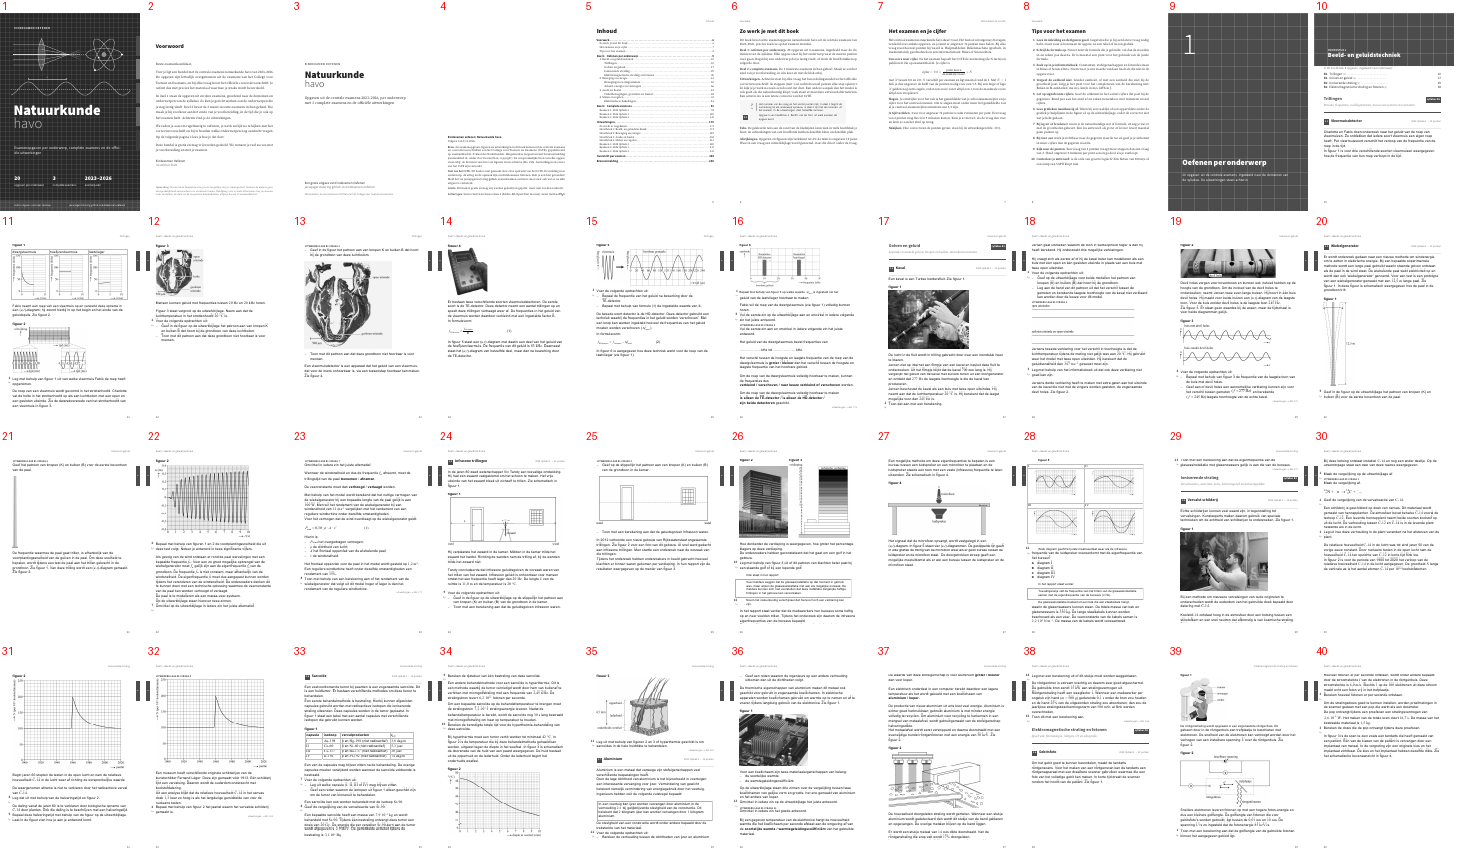
\includegraphics[width=.9\linewidth]{fig/contactvel.png}
\caption{Contactvel van de eerste veertig pagina's van één bundel. Na elke bouw ontstaan per bundel zo'n zeven vellen; zo
zijn alle pagina's visueel geïnspecteerd, aanvullend op de automatische controle.}
\label{fig:contactvel}
\end{figure}

\subsection{Website}
De website is in een latere iteratie heringericht op basis van een marktverkenning van het bestaande gratis aanbod
\cite{markt}. Daaruit bleek dat gratis vragen per onderwerp niet langer onderscheidend zijn, de combinatie van officieel
correctievoorschrift, actualiteit en afwezigheid van account en reclame wel. De herinrichting maakt die kenmerken zichtbaar
(figuur~\ref{fig:site}) en voegt vindbare pagina's per onderwerp, een logboek en een pagina voor docenten toe.

\begin{figure}[!htb]
\centering
\begin{subfigure}[t]{.485\linewidth}\centering
  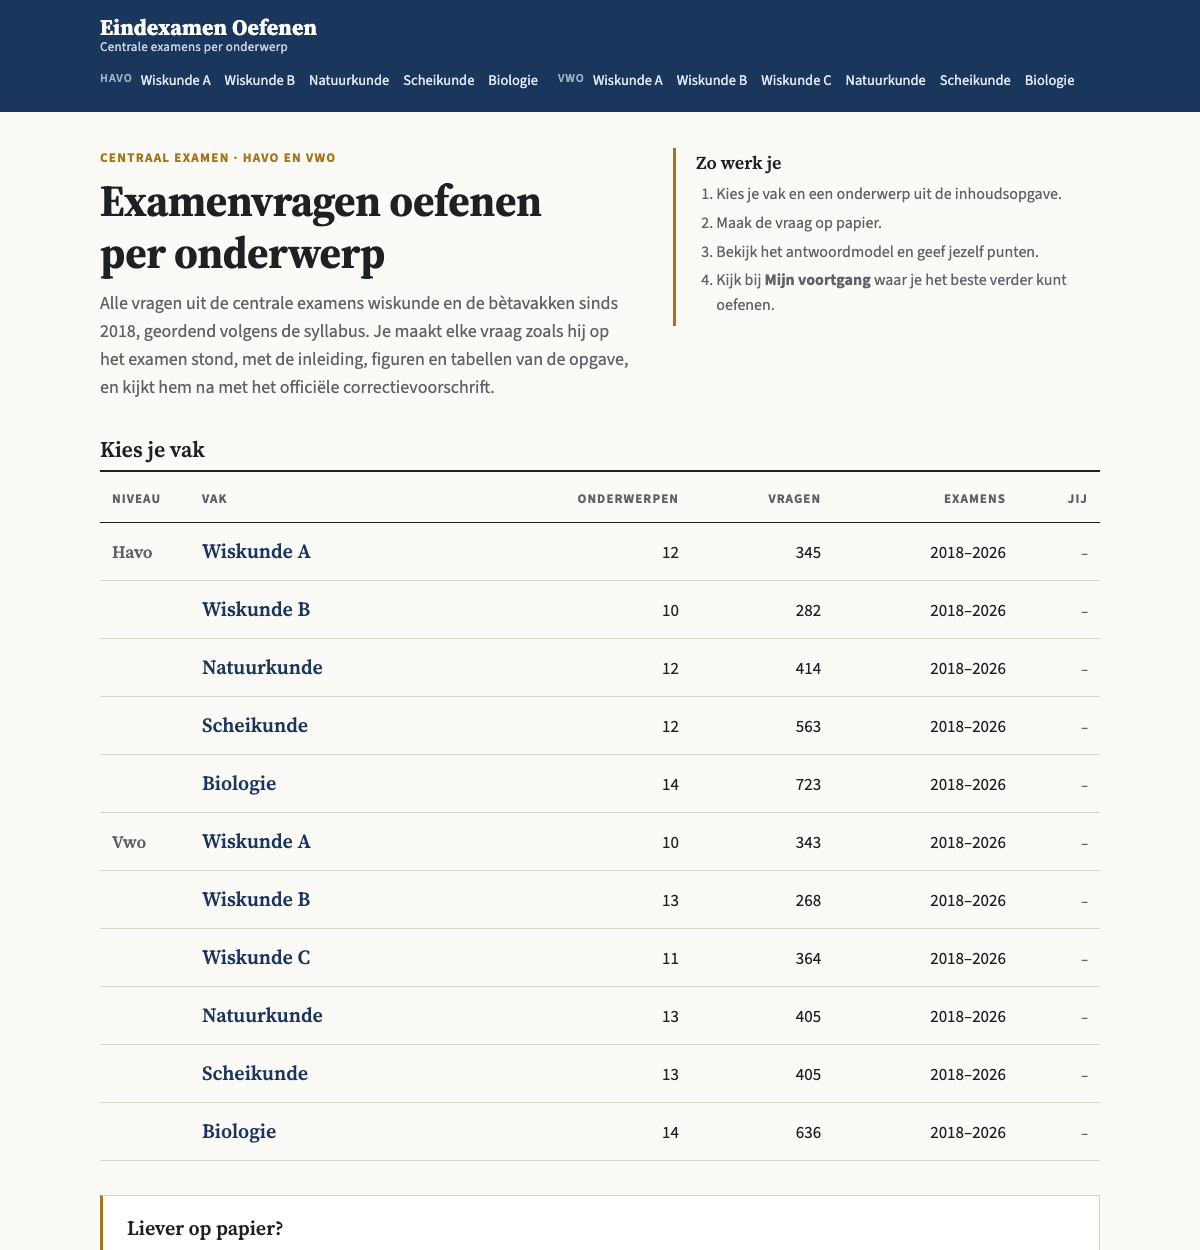
\includegraphics[width=\linewidth,trim=0 330 0 0,clip]{fig/site-voor.png}\caption{Eerste versie.}
\end{subfigure}\hfill
\begin{subfigure}[t]{.485\linewidth}\centering
  
\includegraphics[width=\linewidth,trim=0 330 0 0,clip]{fig/site-na.png}\caption{Na herinrichting.}
\end{subfigure}
\caption{Startpagina voor en na de herinrichting.}
\label{fig:site}
\end{figure}

% =================== 5 ===================
\clearpage
\section{Discussie}

\subsection{Wat nodig was voor een website uit alleen instructies}
Ten aanzien van OV1 laat de casus zien dat de implementatie volledig via natuurlijke taal kon plaatsvinden: de auteur
schreef geen code, en alle producten zijn reproduceerbaar uit de broncode die de agent schreef. Dat betekent echter niet dat
instructies op zichzelf volstonden. Figuur~\ref{fig:randvoorwaarden} vat de randvoorwaarden samen die in deze casus
doorslaggevend waren (OV2).

\begin{figure}[H]
\centering
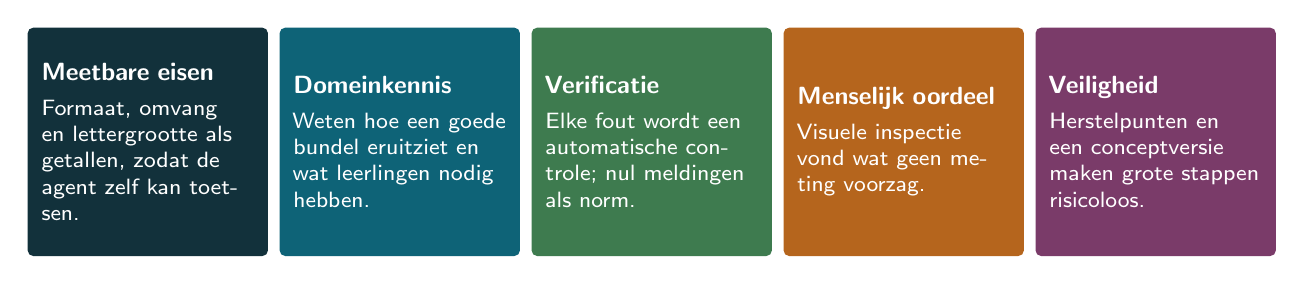
\begin{tikzpicture}[
  blok/.style={fill=#1,text=white,font=\sffamily\footnotesize,text width=27mm,minimum height=29mm,inner sep=5pt,align=left,rounded corners=2pt}]
  \foreach \k/\t/\u [count=\i] in {
      donker/Meetbare eisen/{Formaat, omvang en lettergrootte als getallen, zodat de agent zelf kan toetsen.},
      petrol/Domeinkennis/{Weten hoe een goede bundel eruitziet en wat leerlingen nodig hebben.},
      groen/Verificatie/{Elke fout wordt een automatische controle; nul meldingen als norm.},
      oker/Menselijk oordeel/{Visuele inspectie vond wat geen meting voorzag.},
      pruim/Veiligheid/{Herstelpunten en een conceptversie maken grote stappen risicoloos.}} {
    \node[blok=\k,anchor=north west] at (\i*32mm-32mm,0) {{\small\bfseries \t}\\[3pt]\u};
  }
\end{tikzpicture}
\caption{Randvoorwaarden voor promptgestuurde ontwikkeling, afgeleid uit de casus.}
\label{fig:randvoorwaarden}
\end{figure}

Opvallend is de complementariteit van automatische verificatie en menselijke inspectie. Het controleverslag signaleerde
een groot aantal kleine defecten, maar enkele van de belangrijkste verbeteringen (afgesneden figuren, de nummering, de
wiskundige onjuistheid van de omslag) volgden uit menselijke waarneming en werden pas daarna als meting vastgelegd. Ook de
agent maakte fouten, zoals het onbedoeld beëindigen van een eigen bouwproces en twee gelijktijdige bouwrondes in dezelfde
map; deze werden door de agent gesignaleerd, toegelicht en hersteld.

\subsection{Beperkingen}
Het betreft één casus met één opdrachtgever, die bovendien domeinexpert is; de resultaten zijn niet zonder meer
generaliseerbaar naar opdrachtgevers zonder vakkennis. De indeling van de vragen is door de agent uitgevoerd en
steekproefsgewijs gevalideerd, niet volledig handmatig gecontroleerd. De validatie gebruikt de syllabi van 2026, terwijl de
vragen uit 2018--2026 stammen. Ten slotte is de juridische vraag of het opsplitsen van examens per onderwerp als
``wijzigen'' in de zin van de hergebruikvoorwaarden geldt, niet beantwoord.

% =================== 6 ===================
\section{Conclusie}

Een volledig gratis oefenplatform voor de centrale examens, met website en drukklare bundels, bleek binnen zes dagen
realiseerbaar door één domeinexpert die uitsluitend in natuurlijke taal instrueerde. De kwaliteit werd niet bepaald door de
afzonderlijke instructies, maar door de werkwijze eromheen: meetbare eisen, herstel op systeemniveau, automatische
verificatie en een menselijk eindoordeel. Die werkwijze is niet specifiek voor examens en lijkt toepasbaar op andere
projecten waarin bestaande documenten tot een bruikbaar product moeten worden geordend.

\begin{tcolorbox}[enhanced,colback=donker,colframe=donker,arc=0pt,left=14pt,right=14pt,top=10pt,bottom=10pt,fontupper=\color{white}\small,before skip=12pt]
{\sffamily\bfseries\large Toepassing op andere ideeën}\par\smallskip
Een oefenomgeving, een kennisbank, een rapportage of een boek uit bestaande documenten: wie weet wat het moet worden en voor
wie, kan het op deze manier laten bouwen. Wie wil verkennen wat dat voor een eigen idee betekent, kan contact opnemen via
LinkedIn: \textbf{Jesse Jagers}.
\end{tcolorbox}

\renewcommand\refname{Bronnen}
\begin{thebibliography}{9}\small\setlength\itemsep{1pt}
\bibitem{copyright} College voor Toetsen en Examens, \emph{Copyright en hergebruik van examens}. \url{https://www.examenblad.nl}
\bibitem{claude} Anthropic, \emph{Claude Code}. \url{https://www.anthropic.com/claude-code}
\bibitem{markt} J. Jagers en Claude, \emph{Gratis examenoefenmateriaal in Nederland}, onderzoeksrapport, november 2026.
\bibitem{bundel} ThiemeMeulenhoff, \emph{Examenbundel havo biologie 2022/2023}, inkijkfragment.
\bibitem{site} \emph{Eindexamen Oefenen}. \url{https://jessejagerstutoring.github.io/eindexamen-oefenen/}
\bibitem{repo} Broncode en bouwscripts. \url{https://github.com/jessejagerstutoring/eindexamen-oefenen}
\end{thebibliography}

\end{document}
